\documentclass[a4paper,12pt]{article}

\usepackage[unicode]{hyperref}
\usepackage{cmap}
\usepackage[T2A]{fontenc}
\usepackage[utf8]{inputenc}


\usepackage[verbose,dvips,a4paper,tmargin=20mm,bmargin=20mm,lmargin=20mm,rmargin=20mm,headsep=4pt,includeheadfoot]{geometry}

\usepackage[nodisplayskipstretch]{setspace}
\usepackage{amsmath}
%\usepackage{mathenv}
\usepackage{indentfirst}

\usepackage{txfonts} % use before local fonts - only for math
%\usepackage{dejavu}
\usepackage{atu_csb}
\usepackage{atu_ofs}
\usepackage{atu_nim}

\usepackage{graphicx}
\usepackage{placeins} % FloatBarrier

\usepackage{tikz}
\usetikzlibrary{arrows}
\usetikzlibrary{patterns}
\usetikzlibrary{circuits}
\usetikzlibrary{circuits.ee}
\usetikzlibrary{circuits.ee.IEC}
%\usetikzlibrary{circuits.logic.IEC}

\usepackage[english,ukraineb,russian]{babel}
%\usepackage[margin=10pt,font=small,labelfont=bf,labelsep=endash]{caption} % format=hang|plain...

\tikzset{
  >=stealth,
  %semiRed/.style={fill=red,opacity=0.3,draw=black,thin},
  medline/.style={draw=black,line width=0.6pt},
  boldline/.style={draw=black,line width=2.0pt},
  wire/.style={draw=black,line width=1.0pt},
  elelem/.style={draw=black,line width=1.5pt}
}

\hypersetup{
  pdftitle={Словеса об идентификации},
  pdfauthor={А.И.~Гуда},
  colorlinks=true,
  linkcolor=blue,
  citecolor=brown
}

% \linespread{1.3} setspace must be better
% \onehalfspacing
\setstretch{1.2}

\newcommand{\LinkRef}[1]{ \textit{#1} }


\title{Словеса об идентификации}
\author{А.И.~Гуда}

\begin{document}

% \maketitle
{ \tiny \verb! ~/proj/id_data/text/tasks.tex! }

\tableofcontents


\section{Определение идентификации}

\subsection{История}

Предельные случаи: Заде, Райбман.

L.A.~Zadeh (1956), ``On the Identification Problem,''
IRE Transactions on Circuit Theory, 3, pp.  277--281.

More: Eykhoff, Rastrigin.

\subsection{Новые определения}

Привязка к текущей задаче, физика.

Разные определения для разных задач или свести к одному определению?

\subsection{Критерии идентификации}

\subsubsection{Отличие задачи идентификации от поиска экстремума}

На первый взгляд, при заданном критерии идентификации, задача идентификации
сводится к классической задаче описка экстремума: надо найти такие значения
параметров, при которых критерий принимает максимальное значение.
На самом деле, существуют определённые аспекты, которые делают такое
сведение практически невозможным.

Прежде всего, в задаче поиска
экстремума предполагается, что наблюдаемая система статична:
значение критерия не зависит от времени, и проведя измерение
в точке один раз, можно к нему не возвращаться.
Напротив, идентификация динамической системы предполагает,
что значение критерия, даже после какого-либо усреднения на конечном
интервале времени, есть величина динамическая, причём динамика определяется
не только параметрами системы, но и свойствами самой системы измерения,
а также процессом взаимодействия системы измерения с моделями. При этом
возможны весьма нетривиальные результаты, такие как параметрический
резонанс, распространение параметрических волн на множестве моделей и т.д.

Также существенную роль могут играть как шумы измерения, так и побочные
эффекты от процесса фильтрации шумов. Большая часть фильтров приводит к запаздыванию
в процессе измерения, и игнорирование этих явлений может привести
к нарушению устойчивости поиска.

В задаче поиска экстремума предполагается, что не только
значение функции известно точно в каждой точке, но также известны все производные.
В реальные задачах идентификации производные непосредственно
не доступны для измерения, а их оценка требует применения специальных
методов. При этом процесс оценивания производных, как правило,
более чувствителен к шумам измерения, чес собственно измерение.

Далее, в в задачах поиска экстремума не учитывается возможность
смещения экстремума со временем. Напротив, в задачах идентификации
или же изначально предполагается вариабельность параметров, или же
имеются ограничение на время измерения.


Все эти явления делают задачу идентификации более сложной, чем
классическая задача поиска экстремума, чем и обусловлено
существование широкого спектра методов идентификации. Тем не менее,
некоторые алгоритмы, применимые при поиска экстремума, могут быть
полезны при синтезе системы идентификации.






\subsubsection{Измеримые интегральные характеристики сигнала}

Откуда брать.


\subsection{Тестовые системы (хаотические)}

\subsubsection{Лоренц} % _LOR_

\LinkRef{
  lor: ASAU-22, 23, 24, 25, 26. APIR-2012. CSIT-2015. ISDMCI-2014, ISDMCI-2015.
  ITMM-2012, ITMM-2014, ITMM-2015
}

\begin{equation}
\begin{cases}
  \dot{x} = \sigma (y-x ) , \\
  \dot{y} = x (r-z) - y , \\
  \dot{z} = x y - b z .
\end{cases}
\label{atu:eq:lor}
\end{equation}

Критерий
$\overline{x^2}$


Идентифицируемый параметр:
$r \in [ 5; 100 ] $.

Остальные параметры:
$b = 2.66667$, $\sigma = 10$.


\begin{figure}[htb!]
\centerline{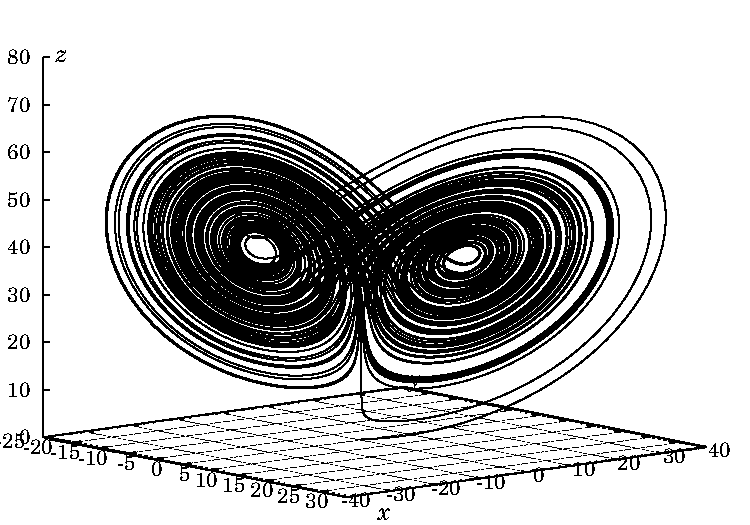
\includegraphics[width=0.5\textwidth]{p/cha/lor_phase3.pdf} }
\caption{Аттрактор системы Лоренца (\ref{atu:eq:lor})}
\label{atu:f:lor_phase}
\end{figure}


\FloatBarrier
\subsubsection{Дуффинг} % _DUFF_

\LinkRef{
 duff: ASAU-12, 15. APIR-2009. \ldots
}

\begin{equation}
 \ddot{x} + c_0 \dot{x} + \Omega_0^2 x + \beta x^3 = u(t) ,
\label{atu:eq:duff}
\end{equation}

\begin{equation}
 m \ddot{x} + \nu \dot{x} + k_1 x + k_3 x^3 = F(t) ,
\label{atu:eq:duff_phys}
\end{equation}

Здесь \(m\) -- масса объекта,
\(x(t)\) -- координата (выходной сигнал),
\(u(t) = U_{in} \sin( \omega_{in} t ) \) -- внешняя возмущающая сила,
\( k_1 \) -- коэффициент линейной компоненты возвращающей силы,
\( k_3 \) -- коэффициент при нелинейной части,
\( \Omega_0 \) -- собственная частота при отсутствии нелинейности,
\( \nu \) и \( c_0\) -- размерный и безразмерный коэффициенты демпфирования,
\( \beta \) -- безразмерный коэффициент нелинейной части.

Идентифицируемый параметр:
$ \beta \approx 2 $.

Остальные параметры:
\(U_{in}=1\), \(\omega_{in}=1\),
\(c_0 = 0.05\), \( \Omega_0 = 1 \).

\begin{figure}[htb!]
\centerline{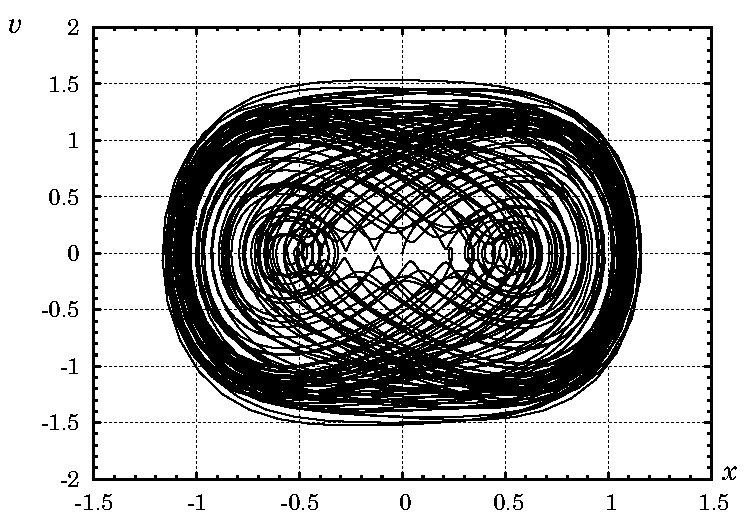
\includegraphics[width=0.5\textwidth]{p/cha/duff_phase.pdf} }
\caption{Фазовый портрет системы Дуффинга (\ref{atu:eq:duff})}
\label{atu:f:duff_phase}
\end{figure}

Критерий
$\overline{x^2}$




\FloatBarrier
\subsubsection{Чуа} % _CHUA_

\LinkRef{
 chua: ASAU-18, MKMM-2014, APIR-2011
}

\begin{figure}[htb!]
\begin{center}
  \begin{tikzpicture}[circuit ee IEC,very thick,circuit symbol unit=3.5mm]
  \node (L1) at (0,1.5) [point up,elelem,inductor={info = $L$}] {};
  \node      at (0.2,2.4) {$I_L$};
  \node (C2) at (1.5,1.5) [point up,elelem,capacitor={info = $C_2$}] {};
  \node      at (1.8,1.8) {$V_2$};
  \node (pc2d) at (1.5,0) [contact] {};
  \node (pc2u) at (1.5,3) [contact] {};
  \node (C1) at (5.0,1.5) [point up,elelem,capacitor={info = $C_1$}] {};
  \node      at (5.3,1.8) {$V_1$};
  \node (pc1d) at (5,0) [contact] {};
  \node (pc1u) at (5,3) [contact] {};
  \node (R) at (3,3) [elelem,resistor={info = $R$}] {};
  \node (Rc) at (7,1.5) [elelem,point up,resistor={info = $R_c$}] {};
  \draw (Rc) ++(-0.15,-0.7) rectangle+(0.3,0.2);
  \draw (L1) |- (pc2d) -- (pc1d) -| (Rc) [wire];
  \draw (L1) |- (pc2u) -- (R) -- (pc1u) -| (Rc) [wire];
  \draw (pc2u) -- (C2) [wire]; \draw (pc2d) -- (C2) [wire];
  \draw (pc1u) -- (C1) [wire]; \draw (pc1d) -- (C1) [wire];
  \node (Gr) at (5,-0.3) [elelem,point down,ground] {};
  \draw (pc1d) -- (Gr) [wire];
  \end{tikzpicture}
\end{center}
\caption{Условная электрическая цепь, реализующая хаотическую систему Чуа}
\label{atu:fig:chuascheme}
\end{figure}


\begin{equation}
\begin{cases}
  C_1 \dot{V_1}  = \frac{1}{R} ( V_2 - V_1 ) - g(V_1), \\
  C_2 \dot{V_2}  = \frac{1}{R} ( V_1 - V_2 ) + I_L, \\
  \dot{I_L}      = - \frac{1}{L} V_2 .
\end{cases}
\label{atu:eq:chua}
\end{equation}

Единственным нелинейным элементом в данной системе является ``диод Чуа'' с
характеристикой $g(V)$~(рис.~\ref{atu:fig:diodchua}),
обладающий различным отрицательным сопротивлением
($m_0$ и $m_1$) на разных участках,
тем самым являющийся управляемым источником энергии.


\begin{equation}
g(V) =
\begin{cases}
  m_1 V = ( m_0 + m_2 ) V & |V| <   U_0, \\
  m_0 V                   & |V| \ge U_0.
\end{cases}
\label{atu:eq:diodchua}
\end{equation}

\begin{figure}[htb!]
\begin{center}
  \begin{tikzpicture}
    \coordinate (XMIN) at (-4.5,0.0);
    \coordinate (XMAX) at ( 4.5,0.0);
    \coordinate (YMIN) at (0,-2.5);
    \coordinate (YMAX) at (0, 2.5);
    \draw (XMIN) -- (XMAX) [medline,->] node[below] {$U$};
    \draw (YMIN) -- (YMAX) [medline,->] node[left]  {$I$};
    \draw (-4,2) -- (-1,1) -- (1,-1) -- (4,-2) [boldline];
    \draw (1,-1) -- (1,0) [dashed,medline];
    \draw (1,-1) -- (4,-1) [dashed,medline];
    \draw (1.41,0) arc [medline,->,start angle=0,end angle=-45,radius=1.41];
    \draw (1,-1) ++(2,0) arc [medline,->,start angle=0,end angle=-18,radius=2.0];
    \filldraw (1,0) circle[radius=0.05,fill=black] node[above] {$U_0$};
    \node[right] at (1.2,-0.6) {$\alpha_1: \tan(\alpha_1)=m_1$};
    \node[right] at (3.0,-1.3) {$\alpha_0$};
  \end{tikzpicture}
\end{center}
\caption{Характеристика \(I=g(V)\) диода Чуа}
\label{atu:fig:diodchua}
\end{figure}


При этом, параметр \(m_0\) определяет поступление энергии в систему
при больших амплитудах \(V_1\), и, в целом, характеризует
энергетические возможности источника.
Аналогично, параметр \(m_1\) определяет поступление энергии
при малых колебаниях, в частности, определяет, будет ли
система переходить в колебательное состояние при малых начальных
возмущениях, и какой будет режим этих колебаний.
С другой стороны, параметр \(m_1\) является суммой
``глобального параметра'' \(m_0\) и ``довеска'',
определяющего дополнительный вклад при малых амплитудах,
то имеет смысл перейти от параметра \(m_1\) к параметру
\( m_2 = m_1 - m_0 \), который тем самым, в целом
и определяет нелинейность
системы. При \( m_2 = 0 \) система становится линейной
и не представляет особого интереса. Поэтому
в данной работе в качестве
идентифицируемого параметра рассматривается параметр \(m_2\).

В зависимости от величины этого параметра,
система может переходить в режимы затухания,
периодического и сложно-периодического движения, а также в режим
хаотических колебаний. При этом сложно-периодическое и хаотическое
движения чередуются с изменением величины \(m_2\).

% Идентифицируемый параметр:
% \( m_2 = m_1 - m_0 \), $ m_2 \in [ -0.1; -0.7 ] $.

Классически параметры задаются следующим образом~[chua]:
$C_1 = 1/9$, $C_2 = 1$, $L= 1/7$, $R = 1/0.7$, $m_0=-0.5$, $ m_2 \in [ -0.15; -1.0 ] $.

Введём обозначения:
\[
  a_{11} = \frac{1}{R C_1}; \;
  a_{13} = \frac{1}{C_1}; \;
  a_{21} = \frac{1}{R C_2}; \;
  a_{23} = \frac{1}{C_2}; \;
  a_{31} = -\frac{1}{L}; \;
  a_g = - \frac{m_0}{C_1}; \;
  \mu = - \frac{m_2}{C_1}.
\]

\noindent
Получаем:

\begin{equation}
\begin{cases}
  \dot{V}_1  = -a_{11} V_1 + a_{11}  V_2  + g_1(V_1) , \\
  \dot{V}_2  = +a_{21} V_1 - a_{21}  V_2  + a_{23} I_L    , \\
  \dot{I}_L  =  a_{31} V_2.
\end{cases}
\label{atu:eq:chua2}
\end{equation}


\begin{equation}
g_1(V) =
\begin{cases}
  ( a_g + \mu ) V , & |V| <   U_0, \\
  a_g V           , & |V| \ge U_0.
\end{cases}
\label{atu:eq:diodchua2}
\end{equation}

При этом классические значения параметров будут представлены следующим образом:
$ a_{11} = 6.5 $, $a_{21} = 0.7$, $ a_{23} = -7 $, $ a_g = 4.5 $,
$ \mu \in [ 1.29 ; 9 ] $.
Соответственно, в этих обозначениях
идентифицируемым параметров является $\mu$.



\begin{figure}[htb!]
\centerline{
  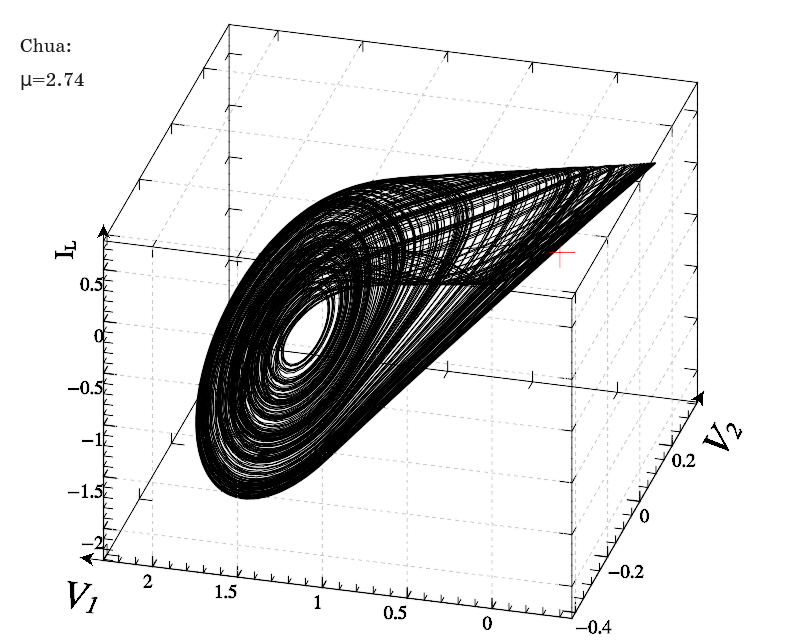
\includegraphics[width=0.49\textwidth]{p/cha/chua/chua_1-p_xyz_mu=2x74.png}
  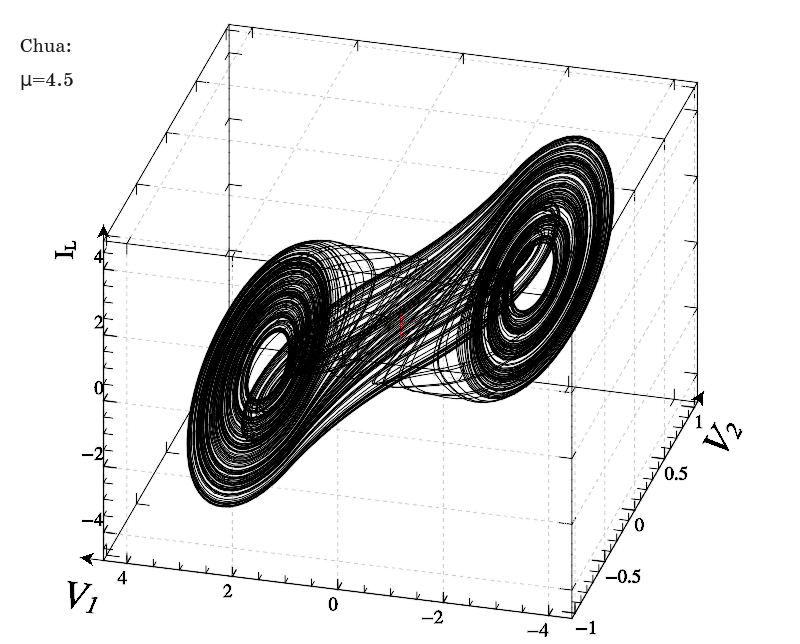
\includegraphics[width=0.49\textwidth]{p/cha/chua/chua_1-p_xyz_mu=4x50.png}
}
\caption{Аттрактор системы Чуа (\ref{atu:eq:chua2}) при различных значениях $\mu$}
\label{atu:f:chua_phase}
\end{figure}

\begin{figure}[htb!]
\centerline{
  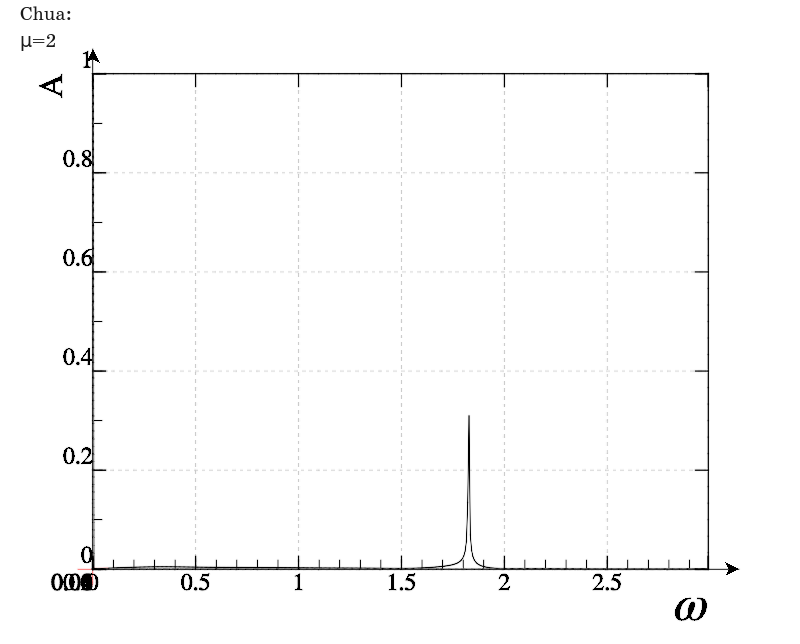
\includegraphics[width=0.32\textwidth]{p/cha/chua/chua_f-p_f_mu=2x00.png}
  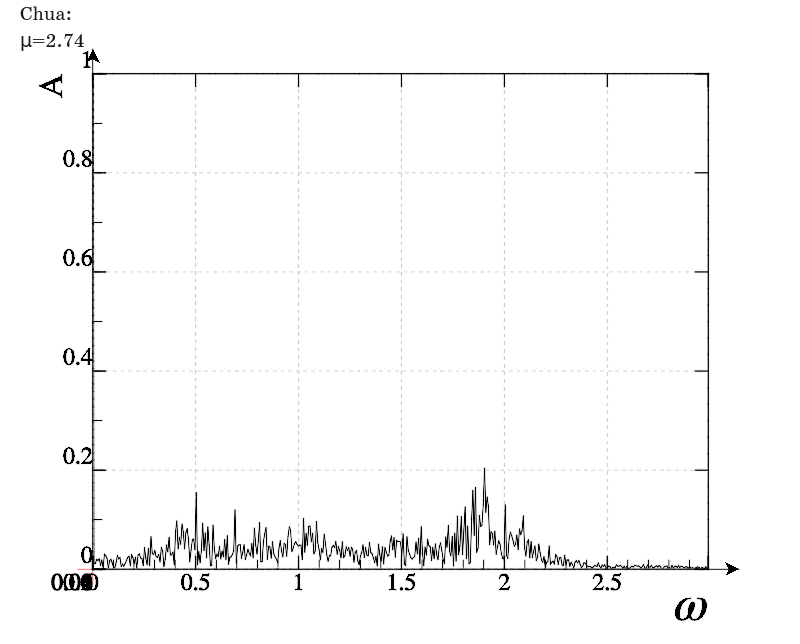
\includegraphics[width=0.32\textwidth]{p/cha/chua/chua_f-p_f_mu=2x74.png}
  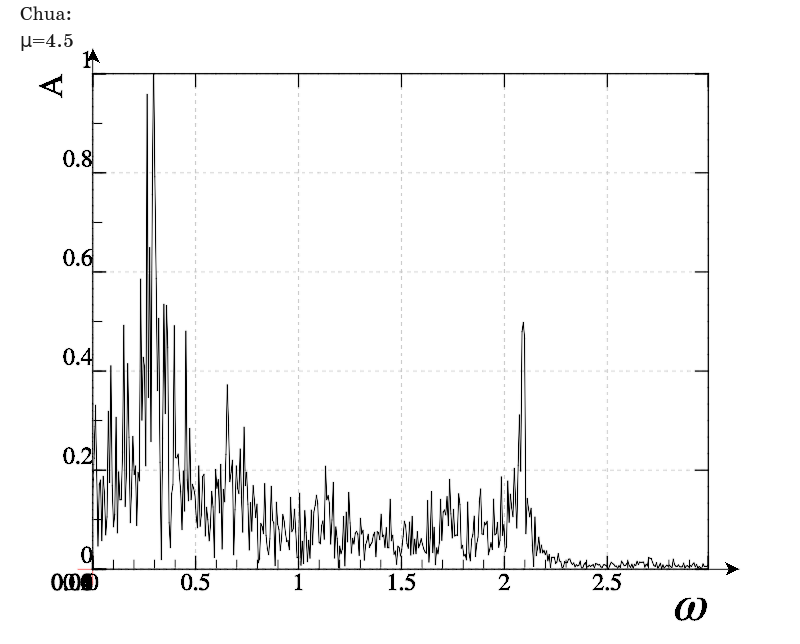
\includegraphics[width=0.32\textwidth]{p/cha/chua/chua_f-p_f_mu=4x50.png}
}
\caption{Спектры системы Чуа (\ref{atu:eq:chua2}) при различных значениях $\mu$}
\label{atu:f:chua_spectrum}
\end{figure}

Для определения критерия рассмотрим зависимости
$q_{*}(\mu) $, полученные путём моделирования
для системы Чуа (рис.~\ref{atu:f:chua_q}):

\begin{figure}[htb!]
\centerline{
  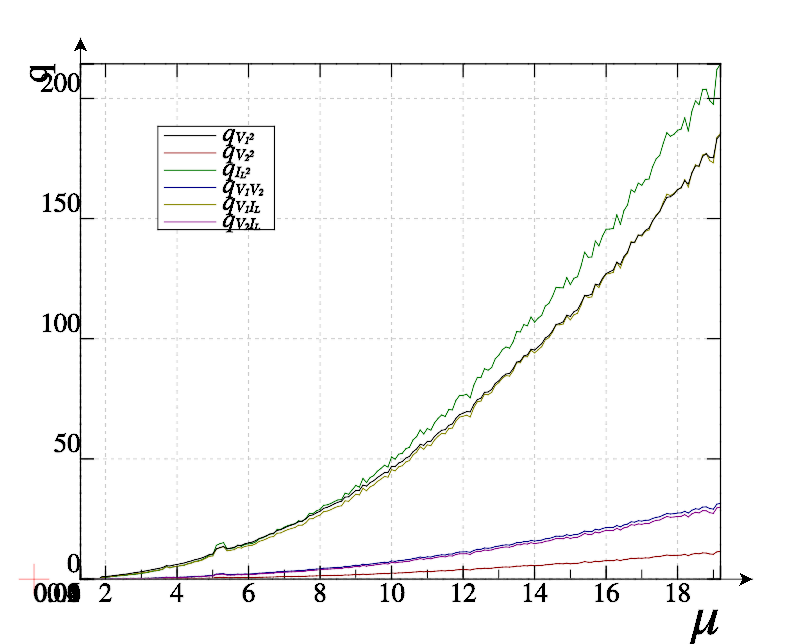
\includegraphics[width=0.49\textwidth]{p/cha/chua/chua_q-p_mu2.png}
  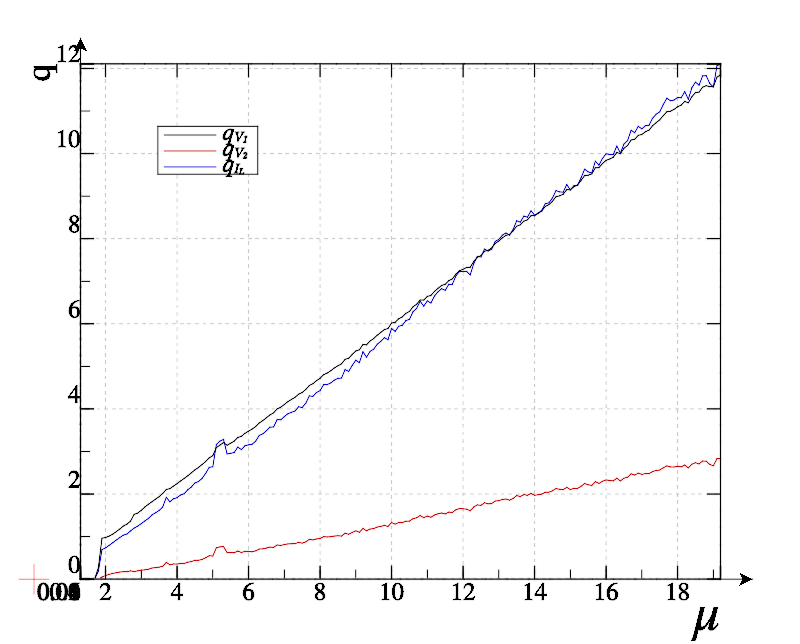
\includegraphics[width=0.49\textwidth]{p/cha/chua/chua_q-p_mu1.png}
}
  \caption{Зависимости $q_{*}(\mu) $ для системы Чуа (\ref{atu:eq:chua2})}
\label{atu:f:chua_q}
\end{figure}

Из графиков очевидно, что величина $ q_{V_1}(\mu) $
является наилучшим кандидатом в критерии, ввиду близкой к линейной зависимости
в рабочем диапазоне.




\FloatBarrier
\subsubsection{Система Рёсслера} % _ROSS_

\LinkRef{
  ross: ASAU-14. ISDMCI-2011, ISDMCI-2012
}

\begin{equation}
\begin{cases}
  \dot{x}  = -y - z  ,  \\
  \dot{y}  = x + a y ,\\
  \dot{z}  = b + z \cdot ( x-c ) .
\end{cases}
\label{atu:eq:rossler}
\end{equation}

Идентифицируемый параметр:
$ c \in [2; 50] $, $c_0=5.88$.

Остальные параметры:
\( a \in (0, 0.35 ) \), $a_0=0.25$,
\(b \in[0;4] \), $b_0=1$.

\begin{figure}[htb!]
\centerline{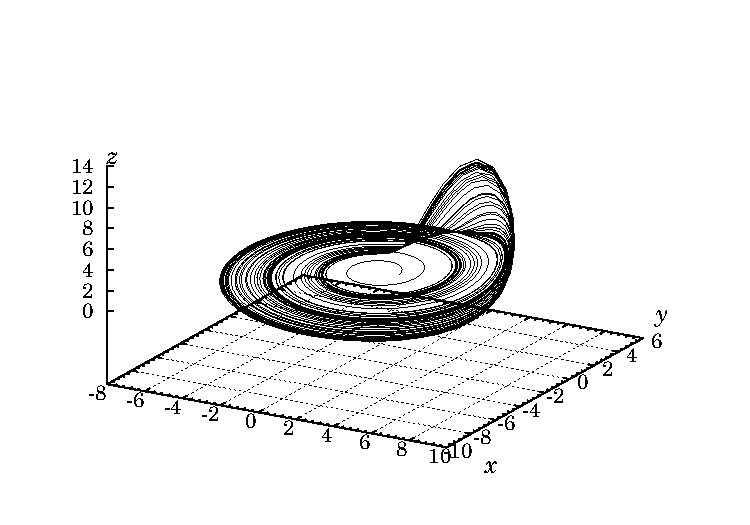
\includegraphics[width=0.5\textwidth]{p/cha/ross_phase3.pdf} }
\caption{Аттрактор системы Рёсслера (\ref{atu:eq:rossler})}
\label{atu:f:ross_phase}
\end{figure}

Критерий
$ z_{\max}$, $ \overline{z} $.



\FloatBarrier
\subsubsection{Ван-Дер-Поль} % _VDP_

\LinkRef{
  vdp: ASAU-16, 17(alt), ITMM-2011
}

\begin{equation}
 \ddot{x} + \varepsilon (1-x^2)  \dot{x} + \Omega_0^2 x  = u(t) .
\label{atu:eq:vdp}
\end{equation}

\( u(t) = U_{in} \sin ( \omega_{in} t ) \),

Идентифицируемый параметр:
\( \varepsilon \in [1;2]  \)

Остальные параметры:
\(U_{in}=0.3\),
\(\omega_{in}=0.2715\).


\begin{figure}[htb!]
\centerline{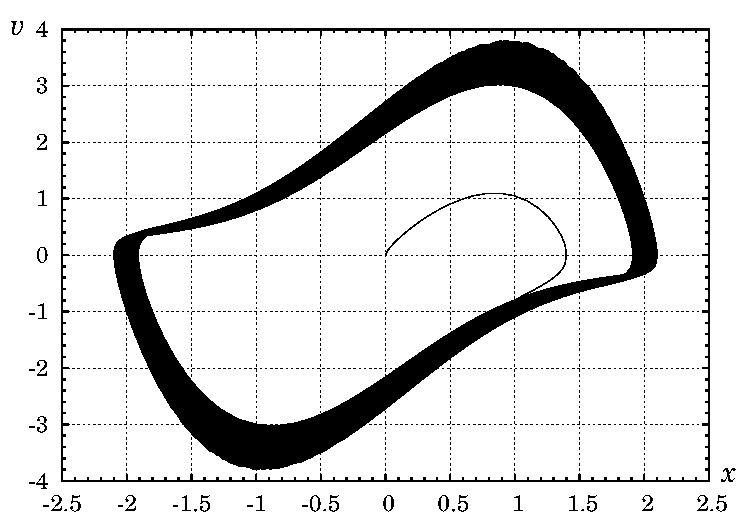
\includegraphics[width=0.5\textwidth]{p/cha/vdp_phase.pdf} }
\caption{Фазовый портрет системы Ван-дер-Поля (\ref{atu:eq:vdp})}
\label{atu:f:vdp_phase}
\end{figure}

Критерий:
$\overline{T}$ + люфт + sign.

Альтернативный критерий:
$\overline{x^2}$


\FloatBarrier
\subsubsection{Колпитц} % _COLP_

\LinkRef{
  colp: ASAU-21, APIR-2013
}

\begin{equation}
\label{atu:eq:colp_phys}
\begin{cases}
  C_1 \frac{dV_{1}}{dt}  = I_L - I_{CE} , \\
  L_1 \frac{dI_L}{dt}    = V_{CC} - V_{1} - V_{2} - I_L R_C , \\
  C_2 \frac{dV_{2}}{dt}  = I_L - \frac{V_{2}}{R_e}.
\end{cases}
\end{equation}

\begin{equation}
\label{atu:eq:colp}
\begin{cases}
  \dot{x} = y - a F(z), \\
  \dot{y} = c - x - by - z, \\
  \dot{z} = y - d z.
\end{cases}
\end{equation}

Используется простая модель транзистора:
\[
F(z) =
\begin{cases}{l}
    e-z-1, \; z \le e-1
    \\
    0, z>e-1
\end{cases}.
\]

Идентифицируемый параметр:
$b \in [ 0.5; 1.1 ]$

Остальные параметры:
$ a = 30$, $b = 0.78$, $c=15$, $d=0.08$, $e=7.5$.

\begin{figure}[htb!]
\centerline{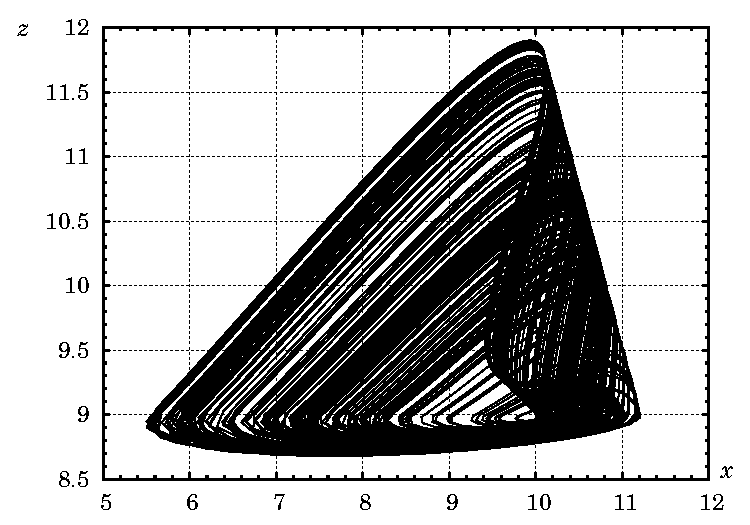
\includegraphics[width=0.5\textwidth]{p/cha/colp_phase.pdf} }
\caption{Аттрактор системы Колпитца (\ref{atu:eq:colp})}
\label{atu:f:colp_phase}
\end{figure}


Критерий
$\overline{y^2}(t)$



\FloatBarrier

\subsubsection{Колебательная с зоной нечувствительности в возвращающей силе} % _DEADVI_

\LinkRef{
  deadvi: ASAU-20, ISDMCI-2013
}

\begin{equation}
\ddot{x} + c_0 \dot{x} + a \cdot x + b \cdot \mathrm{db}(x,x_0) = u(t),
\label{atu:eq:deadvi}
\end{equation}

$ u(t) = U_0 \sin( \omega_{in} t ) $.

Идентифицируемый параметр:
$ x_0 \in [2;2.5] $ -- ширина зоны нечувствительности.

Остальные параметры:
$U_0 = 1.4$, $\omega_{in} = 1.4$, $c_0=0.1$, $a=-0.3$, $b=1.0$.


\begin{figure}[htb!]
\centerline{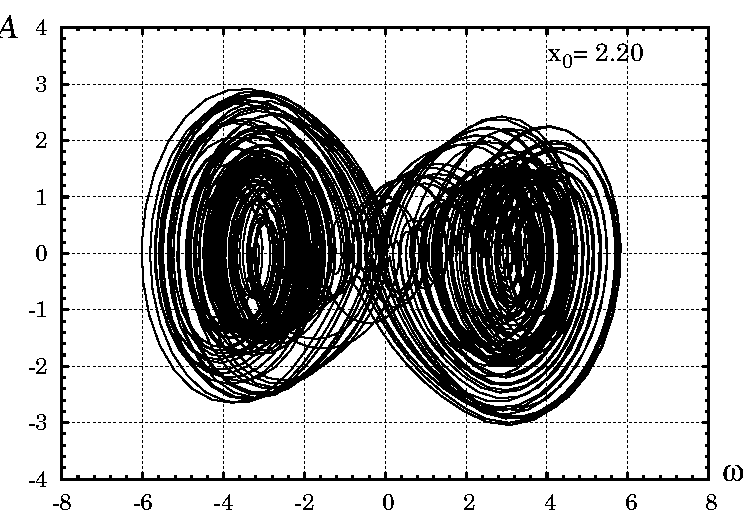
\includegraphics[width=0.5\textwidth]{p/cha/deadvi_phase.pdf} }
\caption{Фазовый портрет системы ``deadvi'' (\ref{atu:eq:deadvi})}
\label{atu:f:deadvi_phase}
\end{figure}

Критерий
$\overline{x^2(t)}$



\FloatBarrier
\subsubsection{Система с сухим трением}

\LinkRef{
  fric: ASAU-11, \ldots
}

\begin{equation}
 m \ddot{x} + f( x, \dot{x}, \ldots)  = u(t).
\label{atu:eq:dryfric_example}
\end{equation}

Критерий
$\overline{e^2(t)}$

Перед этим -- гистерезисная фильтрация.
Или много проще.



\FloatBarrier
\subsubsection{Релаксационные генераторы}


\LinkRef{
  relax: ASAU-18 (no id?)
}

\begin{figure}[htb!]
\centerline{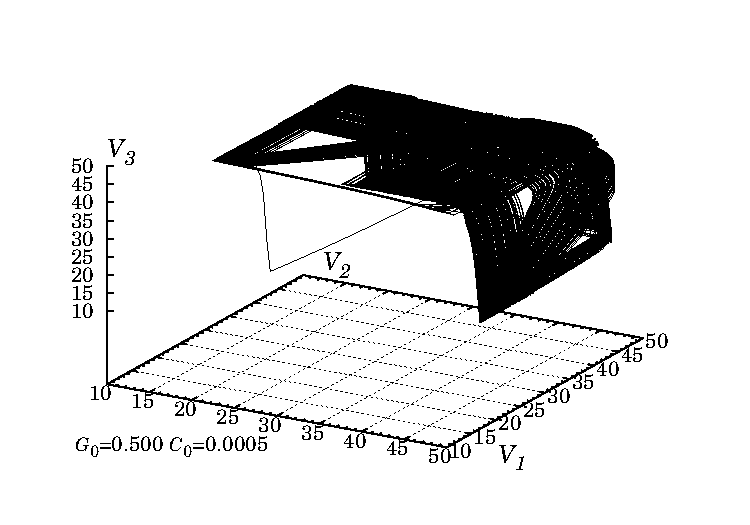
\includegraphics[width=0.5\textwidth]{p/cha/relax_phase3_0500.pdf} }
\caption{Аттрактор системы с релаксационными генераторами}
\label{atu:f:relax_phase3}
\end{figure}



\FloatBarrier
\subsubsection{VGlass} % _VGLASS_

\LinkRef{
  vglass: ITMM-2013
}

\begin{figure}[htb!]
\centerline{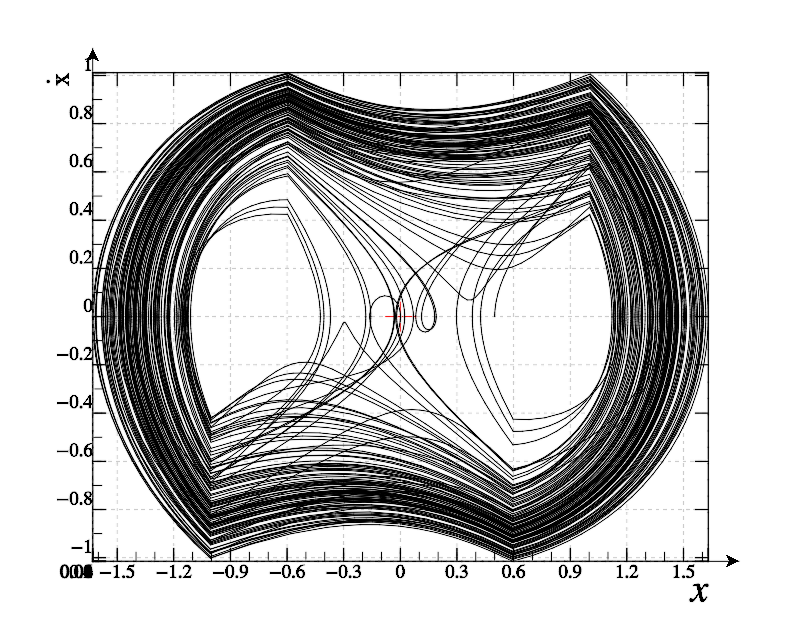
\includegraphics[width=0.5\textwidth]{p/cha/vg1-graph_phase.png} }
\caption{Фазовый портрет системы ``vglass'' }
\label{atu:f:vglass_phase}
\end{figure}

\FloatBarrier
\subsubsection{Sprott A}

\LinkRef{
  sprott\_a: MKMM-2016
}


\FloatBarrier
\subsubsection{Common}

Фрактальные критерии (инвариантные относительно смены частоты дискретизации)?
Надо ли несколько критериев, если параметров несколько.
А может надо, даже если один?

Структуры ...



\FloatBarrier
\section{Методы поиска}

\subsection{Основные параметры поиска}


\subsubsection{Общие свойства объектов с точки зрения идентификации}

\subsubsection{Априорная и текущая информация}

Без априорной информации невозможно построение
работоспособной системы идентификации. Основные
априорные величины определяются на этапе постановки
задачи идентификации. В первую очередь это
параметры масштаба: допустимый диапазон
изменения параметров \( \mathfrak{P}\),
характерное время работы
идентифицируемой системы, а также
требуемая точность и скорость идентификации
(могут быть заданы различными способами).
В этот список входи и максимальная скорость изменения параметра.
В процессе работы эти параметры могут уточнятся по текущей информации.

Следующую часть априорной (по отношению к идентификации) информации
предоставляет процесс синтеза критерия идентификации.
В первую очередь, это сам вид критерия. Им определятся
как диапазон изменения величины этого критерия, так и
динамические свойства: характерное/минимально время
оценивали \(\tau\) (или даже оценка зависимости $\tau$ от точности и других параметров),
характерное время реакции системы на изменение
параметра с учётом динамики измерения \(q\).


\subsubsection{Чувствительность модели}

Убрать или заменить чем-то ещё.


\subsection{Время и история}

Способы учёта истории системы и динамических характеристик.

\subsection{ Использование множества моделей / агентов}

Сколько всего надо моделей? Размер пространства параметров.
Рой, коллектив, главнюк.
Зачем агентам перемещаться?

\textbf{ Агент } -- совокупность модели, критерия идентификации,
алгоритмов поиска и адаптации.

Как правило, один агент управляет одной моделью. При этом
он может использовать информацию, как полученную как от других
агентов, так и полученную в результате обработки данных
всего ансамбля.

\textbf{ Рой } -- множество агентов, обеспечивающее идентификацию за счёт
сосредоточения максимального количества агентов
в области предполагаемого максимума функции качества.
Обычно -- три составляющие поведения
(движение о оцениваемому локальному экстремуму, -- к глобальному, случайная составляющая).

\textit{Для сравнения требуется и это промоделировать.
Достаточно накладно -- надо много агентов.}

Достоинства -- простота алгоритмов.
Недостатки -- требуется избыточное количество агентов.
Значительная часть агентов, находящихся вблизи экстремума,
практически не приносит информации. Роевые
алгоритмы (как и их прообразы в живой природе) ориентированы
для увеличения добычи ресурсов, а не информации.

\textbf{ Ансамбль } -- множество агентов, обеспечивающее идентификацию за счёт
распределения агентов таким образом, который обеспечивает как
точность идентификации за счёт ограниченного скопления агентов
в областях предполагаемых максимумов, так и оперативное переключение
на другие области при изменении параметров за счёт недопущения
неоправданной скученности агентов.

\textit{ Заметная часть новизны планируется здесь}

\subsubsection{Один агент}

Единственный неподвижный агент практически не имеет смысла
с точки зрения синтеза системы идентификации.
Он может сигнализировать о том, что в пределах
\(\tau\) модель была или не была достаточно адекватна
объекту.

Наличие истории и возможность перемещаться дают возможность
построить систему идентификации и на одном агенте.
В качестве истории могут использоваться, в том числе,
динамические свойства идентифицируемого объекта
(оригинальный метод АПИ). Также могут быть
применены интегрирующие элементы агента идентификации
(синхронный детектор, \ldots).

\subsubsection{Пара агентов}

Пара агентов, взаимодействующая между собой,
способна оценить градиент функции качества,
и, следовательно, обеспечить смещение в требуемом направлении.

С учетом глобальной информации возможна адаптация параметров пары.
В свою очередь, информация, полученная от пары может
использоваться для уточнения глобальных параметров.

\subsubsection{Триплет агентов}

Три соседних агента, взаимодействующие между собой,
способны не только оценить градиент функции качества в своей окрестности,
но и определить (опять же, оценочно) наличие там максимума.

\subsubsection{Ансамбль агентов}

\subsection{Адаптация}

Какие параметры системы идентификации можно адаптировать
и на каком уровне.

Когда имеет смысл играть с чувствительностью.

Как близко имеет смысл подводить модели к экстремуму?


Стабильные/мобильные модели.

История: локальная + глобальная

\subsection{Качество идентификации}

Расширить из кандидатской с учётом времени и множества моделей.



\section{Программная реализация}

\subsection{Постановка задачи}

Из того, что получится ;-)

\subsection{Структура программного комплекса}

Комплекс -- потому что несколько программ.
От основной для моделирования, до программ сбора и обработки
информации для микроконтроллеров.

\subsection{Взаимодействие с реальным миром}

Просто прочитать данные - уже работает.
Надо: realtime.
Протокол(ы) взаимодействия (+ существующие).


\section{Реальные задачи}

Ага....


\section{Всякое и старое}



Как надо крутить $\tau_g$ вблизи/вдали
 1) При малом $k_\omega$ сравнить поведение вблизи/вдали при различном $\omega_0$
 2) Двойная инверсия работы генератора?

Две точки усреднения: как объединить? А надо ли?

Адаптация $\tau_q$ / просто $\tau$ от $x$.





\end{document}

